%
If solution exists for the given
system of equations then they
said to be consistent, otherwise they are
inconsistent.
The above equations can be expressed as the matrix equation
\begin{align}
\myvec{1 & 2\\2 & 3} \vec{x} = \myvec{2\\3}
\end{align}
%
The augmented matrix for the above equation and row reducing as follows
\begin{align}
\myvec{1 & 2 & 2 \\ 2 & 3 & 3}  \xleftrightarrow[]{R_2\rightarrow R_2-2R_1} \myvec{1 & 2 & 2 \\ 0 & -1 & -1}\\
\xleftrightarrow[]{R_1\rightarrow R_1+2R_2}
\myvec{1 & 0 & 0\\0 & -1 & -1}\label{aug/2/70/a}\\
\implies\text{Rank}\myvec{1&2\\2&3}=\text{Rank}\myvec{1&2&2\\2&3&3}=2
\end{align}
Here, $Rank(A)=Rank(A|B)$. Therefore, the system is consistent. Also, there exist a unique solution as $Rank(A)=n$ (number of unknown).\\ 
From equation \eqref{aug/2/70/a}, we get:
\begin{align}
    \vec{x}=\myvec{0\\1}
\end{align}
Plotting the lines and the intersection point in Fig.\ref{aug/2/70/b}
\begin{figure}[htp]
\centering
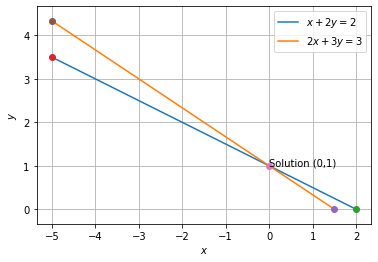
\includegraphics[width=\columnwidth]{solutions/aug/2/70/a_2.png}
\caption{Lines and their intersection denoting the solution}
\label{aug/2/70/b}
\end{figure}
%
$\therefore$ The given system of equation is consistent with unique solution of,
$$\myvec{x\\y}=\myvec{0\\1}$$

